\chapter{Spiking Neural Networks~(SNNs)}
\label{cha:bkg}
The so-called third generation of artificial neural network, spiking neural network (SNN), is comprised of spiking neurons which mimic the dynamics of biological neural behaviour.
In this chapter we will demonstrate the special features of spiking neurons that differ from neurons of conventional artificial neural networks (ANNs);
these biological-plausible neuronal operations are the root of the research problem raised in the thesis: how to operate SNNs to be capable in cognitive tasks as competent as ANNs.
Section~\ref{sec:bio_neuron} will illustrate how biological neurons function and transmit signals between them, the way neural dynamics are modelled by mathematical abstractions as spiking neurons in Section~\ref{sec:spike} , and finally the existing SNN simulators are introduced in Section~\ref{sec:snn_sim}.

\section{Biological Neural Components}
\label{sec:bio_neuron}
%Biological studies have obtained increasing knowledge about facts, functions and anatomy of the brain.
At the cellular level, the central nervous system consists of two types of cells: neurons, the elementary processing units, and glial cells, the structural and metabolic supporters. 
Here we focus on the neurons, since they are the basic elements to build up higher brain functions such as cognition, thought and action. %the path from neurons, neural circuits and networks to behaviour and cognition of the brain.
The human brain contains around a hundred billion ($10^{11}$) such processing units, and up to four orders of magnitudes more connections, ($10^{15}$) all over the brain.
The special structures of neurons enable them to send signals rapidly and precisely to other cells through these connections.
\subsection{Neuron}
	\begin{figure}[bt]
	\centering
	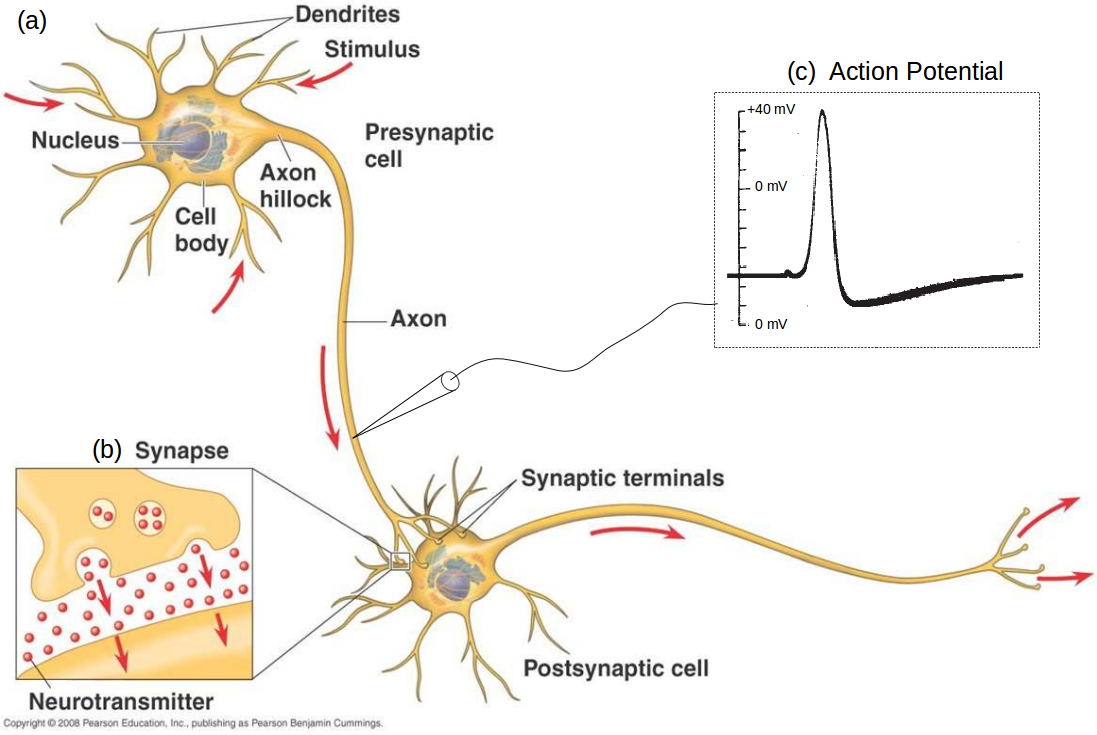
\includegraphics[width=0.98\textwidth]{pics_snn/neuron2.png}
	\caption{Two neurons connected by synapses. 
		A neuron comprises three functional parts: dendrites, the soma, and the axon. (a) A pre-synaptic cell connects to its post-synaptic cell through synapses~\cite{reece2011campbell}, see (b)~\cite{reece2011campbell}, and the neural signal, action potential see (c)~\cite{hodgkin1939action}, propagates along the red arrows. }
	\label{Fig:neuron_basic}
\end{figure}

A typical neuron comprises of three functional parts: dendrites, a cell body (soma), and an axon, see Figure~\ref{Fig:neuron_basic}(a).
The dendrites of a neuron receive stimuli from other neurons, and transmit the neural signal to the neuron's soma.
The soma is the cell body of the neuron, the location of nucleus, and functions as a non-linear processor which triggers an output signal when accumulated total input exceeds some threshold.
The output signal initiates from the axon hillock where the axon emerges from the soma, and is propagated through the axon to other neurons.
Most neurons contains only one axon, but may connect to many neurons by branching out axon terminals. 


The signal delivery from one neuron to another occurs at the junction between these two neurons, which is called a synapse, see Figure~\ref{Fig:neuron_basic}(b).
The configuration can be seen as a pre-synaptic cell which sends the signal, and a post-synaptic cell which receives.

%Spiking neuron models can be divided into two major categories \cite{gernstbook} based on their level of abstraction: The conductance models and the threshold models.
%The conductance models simulate a lower level on the ion channels, while the threshold models represent a higher level of neuron abstraction where the threshold voltage is fixed and the neuron fires once the membrane potential reaches it.
%
%In general, Conductance-Based models have been derived from the Nobel prize winners (1963) Hodgkin and Huxley, based on the experiments that they performed on the giant axon squid \cite{hhmodel}.
%Spikes arriving at a LIF neuron cause a temporary flow of current into (excitatory synapse) or out of (inhibitory synapse) the neuron, modelling the behaviour of synapses in biological neurons.
%The LIF neuron sums up this current over time, accumulating charge which gradually leaks away.
%If the membrane potential in the neuron reaches a certain threshold, it produces a spike and its charge is reset.
%LIF neurons have been extensively used in large spiking neural networks \cite{Delorme1999989} because of their ease of implementation and the low computational cost.


\subsection{Neuronal Signals}
Neuronal signals propagated among neurons are short electrical pulses, and Figure~\ref{Fig:neuron_basic}(c) shows the original recording of such a so-called \textbf{action potential} observed on using an squid giant axon.
A typical action potential, also known as a `\textbf{spike}', is of about 100~mV amplitude and lasts 1-2~ms.
Usually, there is a time period immediately after a spike that the neuron is unresponsive to any further stimulus.
This minimal time difference between two spikes of a single neuron is the absolute refractory period during which no spike can be generated.
After the absolute refractory period, it is still difficult but possible to 
fire a spike during the relative refractory period.

The size and duration of the spikes do not vary much among different species, and maintain the same form as the electrical pulses propagates along the axon as illustrated in Figure~\ref{Fig:neuron_basic}(c).
Therefore, the form of an action potential carries little information;
it is the frequency and timing of the spikes that encode the messages.
A sequence of action potentials generated by a single neuron is called a spike train, which can be seen as binary events against discrete time where `on' indicates a spiking event whereas `off' means none.
Information can be encoded in the frequency and timing of these binary events.


The rate coding model states that the spiking rate represents the intensity of a stimulus, e.g. as the stimulus becomes stronger, the frequency of the action potentials also increases.
An example of the tuning curve of a V1 (visual area one of the visual cortex) simple cell responding to different stimulus orientation is shown in Figure~\ref{Fig:v1}.
As the stimulus becomes more aligned to the preferred orientation ($0^\circ$) of the neuron, the firing rate increases.

\begin{figure}[bt]
	\centering
	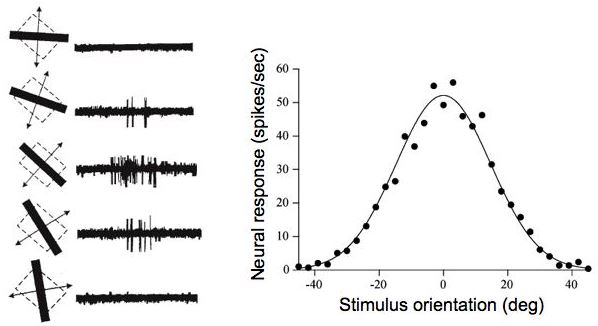
\includegraphics[width=0.9\textwidth]{pics_snn/v1.jpg}
	\caption{Example of rate coding: spike trains for different stimulus orientation (left) of a V1 simple cell of a cat, and the tuning curve (firing rate against stimulus orientation) of the neuron (right)~\cite{hubel1962receptive}.
	The square indicates the visual receptive field of the neuron, and a bar is placed at different orientations and moves to the direction perpendicular to its orientation.
    As the stimulus becomes more aligned to the preferred orientation ($0^\circ$) of the neuron, the firing rate increases.}
	\label{Fig:v1}
\end{figure}

Rate coding works well when the stimulus is changing slowly and the observation time period is long enough to estimate the firing rate, however in practice the stimulus, e.g. visual sensory input, varies in a fast time scale and the neurons respond within a short reaction time.
Thus, temporal coding, encoding information into the precise timing of spikes, is a candidate method to compensate the encoding of fast changing stimulus.

Sound localisation requires temporal coding at sub-millisecond precision, which is a good example of one of the temporal coding schemes, phase locking.
Figure~\ref{Fig:audio_fibre} shows phase-locked spike trains generated by Inner Hair Cells in the cochlea.
Phase locking forms the basis
of detecting time differences of binaural sound inputs.
\begin{figure}[bt]
	\centering
	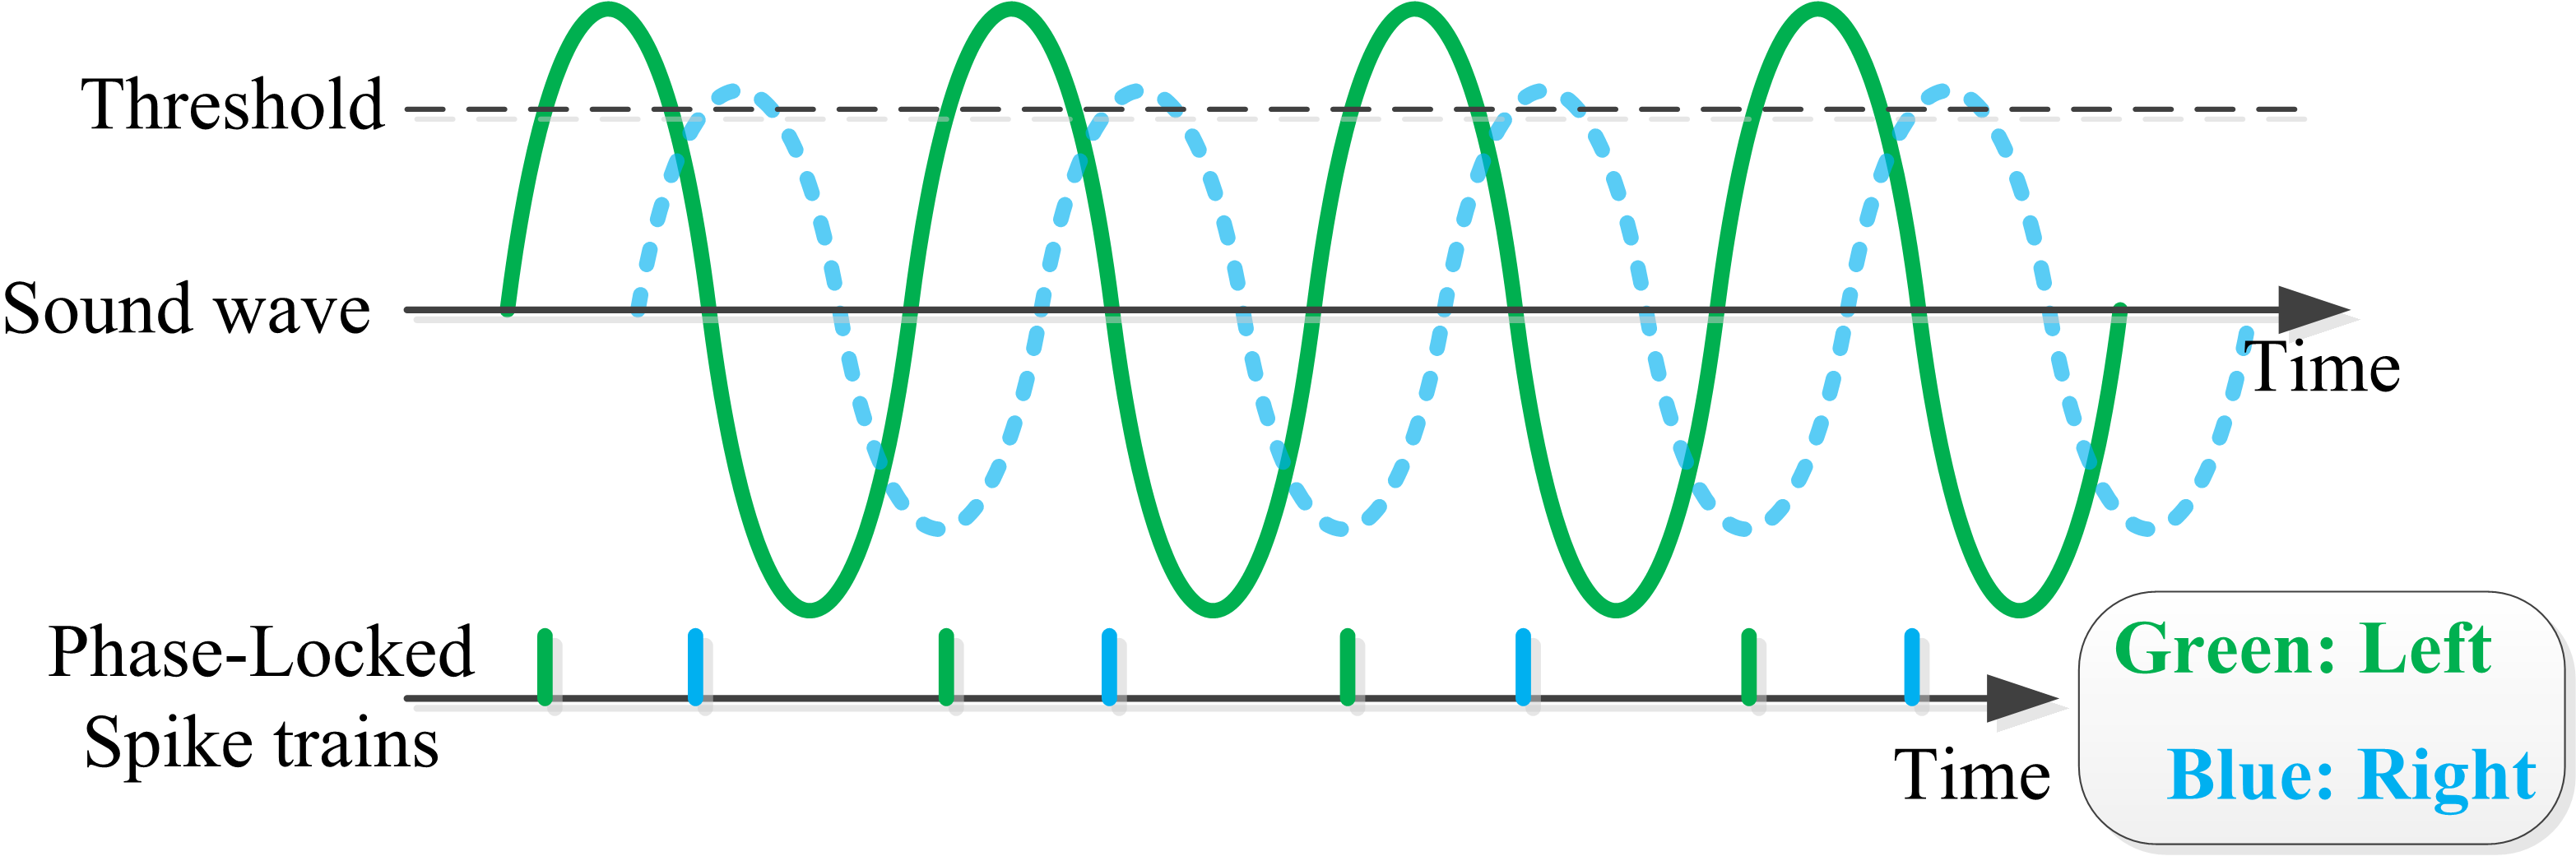
\includegraphics[width=0.9\textwidth]{pics_snn/phaselocking.png}
	\caption{Example of temporal coding: phase-locked spike trains generated by Inner Hair Cells in the cochlea~\cite{liu2013modeling}.
	A sound source generates a sine wave of a certain frequency and conducts to two ears with a time difference and different amplitude due to the angle and distance of the sound source to the head.
	Two spike trains respond to different phases manipulated by a threshold of the sound waves.
	Sound localisation should be resolved by calculating the time difference and level difference of these sound waves which are encoded in the spike trains.
    }
	\label{Fig:audio_fibre}
\end{figure}

Time-to-first-spike encodes the information according to the intensity of a stimulus where a spike shortly after a reference signal indicates a strong stimulation and a later action potential is interpreted as a weaker input.
The tactile afferent information generated by forcing fingerprints from various directions are encoded in such a time-to-first-spike coding scheme~\cite{johansson2004first}.
Synchrony coding also can be found in the brain, where neurons represent the same `concept' always fire at the same time~\cite{von1994correlation}, for example in object recognition~\cite{gray1989stimulus}.
Established from the context of fast object recognition, rank-order coding was proposed where the precise time of spikes is discarded, but rather uses the relative order of spikes among a group of neurons~\cite{gautrais1998rate}.


\subsection{Signal Transmission}
\label{subsec:spike_trans}
The spike, as an electrical signal, propagates to another neuron at the junction between these two neurons, a chemical synapse.
The axon terminal of a pre-synaptic neuron approaches very close (about 20~nm) to the dendrites (or cell body) of a  post-synaptic neuron.
The tiny space between neurons at a synapse is called the synaptic cleft, which is illustrated in Figure~\ref{Fig:neuron_basic}(b).
At such a chemical synapse, the action potential generated by the pre-synaptic neuron triggers chemical neurotransmitter molecules to be released into the synaptic cleft, and once the post-synaptic neuron detects these neurotransmitters it opens specific ion channels to allow electrical current in.
Hence, synapses complete the transformation from electrical signal to chemical molecules and then back to ion influx.
The amount of neurotransmitter determines the strength of the current flow into the post-synaptic neuron.
Thanks to synaptic plasticity, changes of chemical synapses enables modulations on the synaptic efficacy, and forms the neuronal correlation of learning and memory.

\section{Modelling Spiking Neurons}
\label{sec:spike}

\subsection{Neural Dynamics}
%\subsubsection{Membrane Potential}

\begin{figure}[tb!]
	\centering
	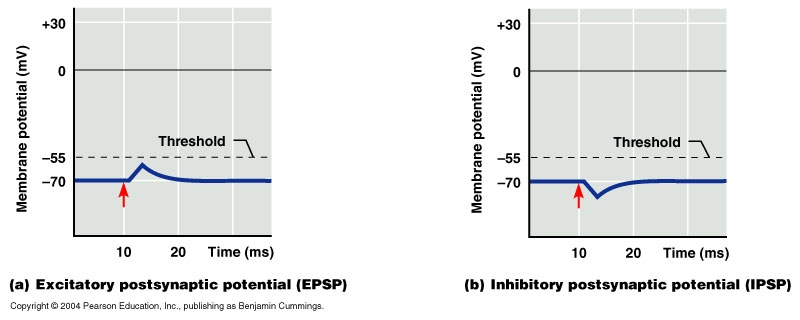
\includegraphics[width=0.98\textwidth]{pics_snn/EI_PSP.JPG}
	\caption{Post-synaptic potential driven by a spike, where the red arrow represents a spike arriving at the neuron~\cite{marieb2007human}.}
	\label{Fig:psp}
\end{figure}

The effect of an ion influx on the post-synaptic neuron caused by spike transmission is a change of potential difference between the interior and exterior of the cell body, and is called the \textbf{membrane potential}.
The membrane potential of a post-synaptic neuron stays at a \textbf{resting potential} in the absence of an input.
As soon as a spike arrives, the membrane potential will be either depolarised (increased) or hyper-polarised (decreased) according to the type of synapse, and go back to the resting potential driven by the membrane leakage.
The state of the membrane potential change caused by a single spike is called the post-synaptic potential (\textbf{PSP}). 
Thus, a spike transmitted by an excitatory synapse triggers a positive change of PSP, named excitatory post-synaptic potential (\textbf{EPSP}), see Figure~\ref{Fig:psp}(a);
a negative change, inhibitory post-synaptic potential (\textbf{IPSP}), is driven by inhibitory synaptic event and is shown in Figure~\ref{Fig:psp}(b).
Spikes arriving at different synapses at the same post-synaptic neuron have PSPs of different amplitudes according to the synaptic efficacy.

%\begin{figure}[tbh!]
%	\centering
%	\begin{subfigure}[t]{0.8\textwidth}
%		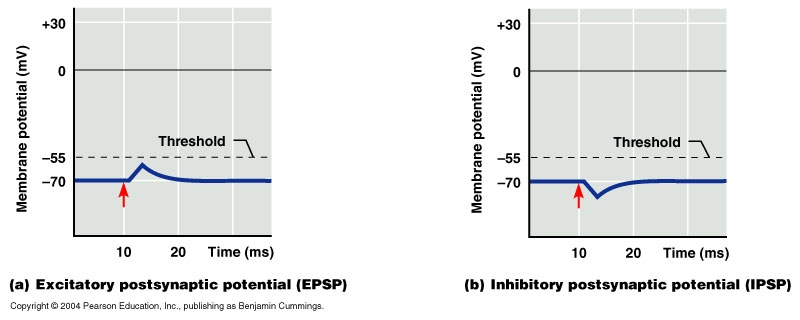
\includegraphics[width=\textwidth]{pics_snn/EI_PSP.JPG}
%		\caption{An electrode measures the \textbf{membrane potential} of a post-synaptic neuron which connected by two pre-synaptic neurons.}
%	\end{subfigure}\\
%	\begin{subfigure}[t]{0.8\textwidth}
%		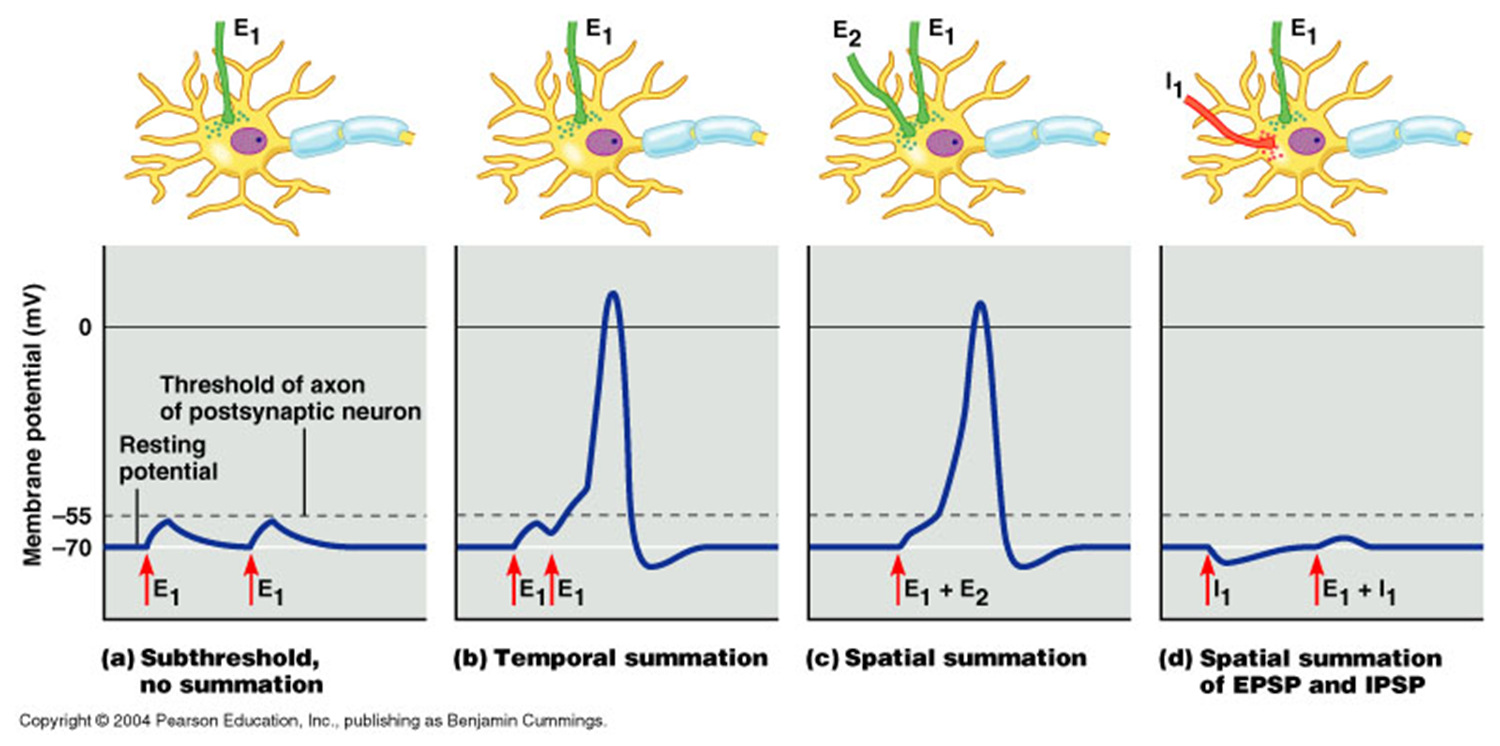
\includegraphics[width=\textwidth]{pics_snn/psp.png}
%		\caption{\textbf{post-synaptic potential (PSP)} generated by spikes of its pre-synaptic neurons adds up to its \textbf{membrane potential} change. }
%	\end{subfigure}
%	\caption{A post-synaptic neuron $i$ receives input from two pre-synaptic neurons $j=1,2$.}
%	\label{Fig:neural_dynamics}
%\end{figure}



\begin{figure}[bt!]
	\centering
	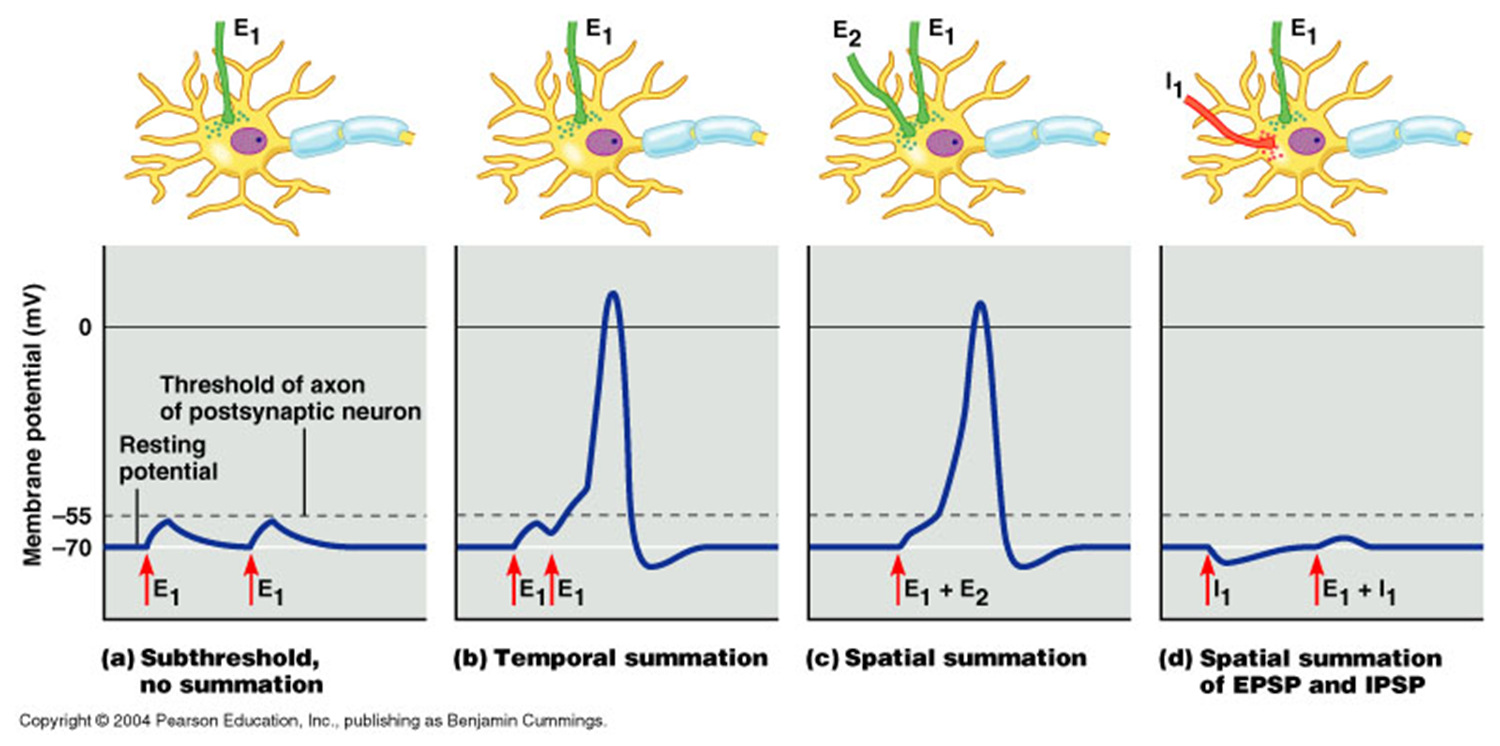
\includegraphics[width=0.9\textwidth]{pics_snn/psp.png}
	\caption{Summation of post-synaptic potentials~\cite{reece2011campbell}. 
		(a) Single EPSPs are usually not strong enough to trigger an action potential without summation. (b) Temporal summation of two EPSPs of the same synapse generates an action potential. (c) Spatial summation of two EPSPs of two synapse generates an action potential. (d) Spatial-temporal summation of both EPSP and IPSPs.
	}
	\label{Fig:psp_sum}
\end{figure}

Singe PSPs have an accumulative effect on the membrane potential both in temporal and spatial.
The accumulation performs simple summation of PSPs until the membrane potential reaches a \textbf{threshold}, when an action potential will be generated at the post-synaptic neuron.
Figure~\ref{Fig:psp_sum} illustrates temporal and spatial summations of PSPs under different circumstances.

Neural dynamics of the membrane potentials, PSPs, and spike trains are all time dependent, while neurons of ANNs, e.g. sigmoid units, only cope with numerical values representing spiking rate, without timing information, see Figure~\ref{Fig:compare_as}.
A regular artificial neuron (Figure~\ref{Fig:compare_as}(a)) composes a weighted summation of input data, $\sum x_i w_i$, and an activation function, $f$, applying on the sum. Usually, a bias is included in the weighted summation which can be seen as an extra input $x_b = 1$ with its weight set to $b$.
However, in this thesis we exclude biases for both artificial and spiking neurons to simplify neural models and to reduce parameters.
Thus the input of a spiking neuron (Figure~\ref{Fig:compare_as}(b)) are spike trains generated by pre-synaptic neurons, which creates PSPs on a post-synaptic neuron and triggers a spike train as the output of this spiking neuron.
These fundamental differences on input/output representation and neural computation lead to special model descriptions of spiking neurons (illustrated in the next section), and raises the research problem of how to operate and train biological-plausible SNNs to be competent in cognitive tasks just as ANNs.

	\begin{figure}[tb!]
		\centering
		\begin{subfigure}[t]{0.28\textwidth}
			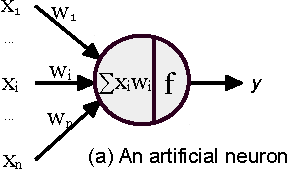
\includegraphics[width=\textwidth]{pics_snn/neuron_ann.pdf}
			%			\caption{Current sampled at $dt$=1~ms.}
		\end{subfigure}~
		\begin{subfigure}[t]{0.65\textwidth}
			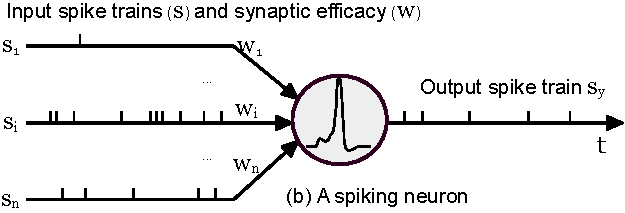
\includegraphics[width=\textwidth]{pics_snn/neuron_snn.pdf}
			%			\caption{Current sampled at $dt$=10~ms.}
		\end{subfigure}
		\caption{Comparisons of processing mechanisms of an artificial and a spiking neuron. (a) An artificial neuron takes numerical values of vector \textbf{x} as input, works as a weighted summation followed by an activation function $f$. (b) Spike trains flow into a spiking neuron as input stimuli, trigger linearly summed-up PSPs through synapses with different synaptic efficacy \textbf{w}, and post-synaptic neuron generates output spikes when membrane potential reaches some threshold.}
		\label{Fig:compare_as}
	\end{figure}
	
\subsection{Neuron Models}
\label{subsec:neuron_model}
The keys of modelling a spiking neuron are: 
\begin{itemize}
	\item to mathematically formalise the evolution of membrane potential;
	\item to state a mechanism of spike generation.
\end{itemize}

\subsubsection{Leaky Integrate-and-Fire}
The evolution of membrane potential can be simplified as a resistor-capacitor (RC) circuit which consists of a membrane capacitor, $C_m$ and a membrane resistance $R_m$, both driven by input current flow $I$, see Figure~\ref{Fig:rc}.
In the resting state without any input, the membrane potential $V$ stays at the same potential as the battery $V_{rest}$.
When current flows into the neuron, it will charge the capacitor with current $I_C(t)$ and discharge through the resistance with current $I_R(t)$ to depolarise the membrane potential when the input current stops and the capacitive charge will decay back to $V_{rest}$ by leaking through the resistance:
\begin{equation}
\begin{aligned}
	I(t) &= I_R(t) + I_C(t) \\[10pt]
	&= \dfrac{V-V_{rest}}{R_m} + C_m \dfrac{\D V}{\D t}~~.
\end{aligned}
\label{equ:LIF_current}
\end{equation}
The standard form of the LIF model describes the sub-threshold membrane potential evolution:
\begin{equation}
	\tau_m \dfrac{\D V}{\D t} = -(V-V_{rest}) + R_m I(t)~,
\end{equation}
where $\tau_m = C_m R_m$ is called the membrane time constant, and as soon as the membrane potential reaches the threshold $V_{thresh}$, it is set to a reset potential $V_{reset}$, which is usually lower than $V_{rest}$: 
\begin{equation}
V = V_{reset}~.
\end{equation}

\begin{figure}[tb!]
	\centering
	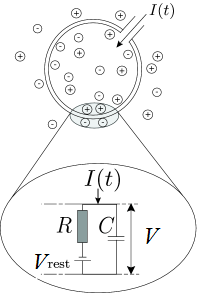
\includegraphics[width=0.3\textwidth]{pics_snn/RC.png}
	\caption{Current flowing into a neuron functions like a resistor–capacitor (RC) circuit~\cite{gerstner2014neuronal}.}
	\label{Fig:rc}
\end{figure}
The simple LIF model uses: (1) a linear differential equation to describe the evolution of membrane potential;
and (2) a threshold to generate a spike.
%\begin{equation}
%V(t) = V_{reset} + R_m I(t) + (V(0) - V_{reset}) - R_m I(t)) e^{-t/\tau_m}.
%\end{equation}

\subsubsection{Hodgkin-Huxley}
Hodgkin-Huxley is the Nobel Prize winning model that explains ionic mechanisms generating and transmitting action potentials in the squid giant axon~\cite{hodgkin1939action}.
The current $I_R(t)$ which flows through the membrane resistance is determined by three ion channels: a leak channel with a conductance of $g_L$, the sodium channel of $g_{Na}$ conductance and the potassium channel of  $g_{K}$ conductance.
The currents which flow through these channels are all proportional to the difference between the membrane potential and the reversal potentials of the channels: $V-E_L$, $V-E_{Na}$, and $V-E_{K}$ respectively.
Thus Equation~\ref{equ:LIF_current} is detailed as:
\begin{equation}
\begin{aligned}
I(t) &= I_L(t) + I_{Na}(t) + I_{K}(t)+ I_C(t) \\
&= g_L(V-E_L) + g_{Na}m^3h(V-E_{Na}) + g_{K}n^4(V-E_{K})  + C_m \dfrac{\D V}{\D t}~~.
\end{aligned}
\label{equ:HH_current}
\end{equation}
 
The Hodgkin–Huxley model can be seen as a non-linear differential equation with four state variables, $V$, $m$, $h$ and $n$ that change against time:
\begin{equation}
\begin{aligned}
C_m \dfrac{\D V}{\D t} = I(t) - g_{K}n^4(V-E_{K}) &- g_{Na}m^3h(V-E_{Na}) - g_L(V-E_L)~, \textrm{~~and }\\[10pt]
\dfrac{\D m}{\D t} &= \alpha_m(V)(1-m) - \beta_m(V)m~, \\[10pt]
\dfrac{\D n}{\D t} &= \alpha_n(V)(1-n) - \beta_n(V)n~, \\[10pt]
\dfrac{\D h}{\D t} &= \alpha_h(V)(1-h) - \beta_h(V)h~,
\end{aligned}
\end{equation} 
where $\alpha(V)$ and  $\beta(V)$ are empirical functions of membrane potential.
With regard to the mechanism of spike initiation, it refers to the most significant property of the Hodgkin-Huxley model that the model is able to generate action potentials with the changes of those dynamic internal variables alone.

The Hodgkin-Huxley equations provides a detailed, quantitative, and reasonable accurate mathematical model explaining the evolution of the membrane potential and the action potential~\cite{byrne2014molecules}.
However, its numerical complexity and highly non-linear characteristics prohibit it from being intuitively understood and make large-scale simulations too expensive.
Therefore, neural model selection should take account of objectives, degree of detail and computational power.

\subsubsection{Izhikevich}
The Izhikevich model is proposed to solve the problems of computational complexity of the Hodgkin-Huxley model and the insufficient capability of LIF model to reproduce the complex dynamics of cortical neurons~\cite{izhikevich2003simple}.
Thus the model can be employed to simulate large-scale brain models comprising of real biological neurons.

The membrane potential evolves in accordance with a pair of differential equations:
\begin{equation}
\begin{aligned}
\dfrac{\D v}{\D t} &= 0.04v^2 + 5v + 140 - u - I(t)~,\\[10pt]
\dfrac{\D u}{\D t} &= a(bv - u)~,
\end{aligned}
\end{equation}
where $v$ is the membrane potential and $u$ represents the membrane recovery which negatively feeds back to $v$.
In terms of spike generation, the initiation part of an activation potential is produced by the equations, but a resetting scheme is needed:
\begin{equation}
\left\{
\begin{aligned}
v &= c \\
u &= u + d
\end{aligned}
\right.
\textrm{~~~~when~} v \geq 30.
\end{equation}  
$a$, $b$, $c$, and $d$ are constant parameters that can be configured to reproduce various neural dynamics of real biological neurons~\cite{izhikevich2004model}.

\subsection{Synapse Model}
Applying spiking neuron models to synaptic spike transmission, we can use two types of synapses: current-based and conductance-based models.
Thus the synaptic efficacy $w$ determines either the input current intensity flowing through the synapse: % (current-based model)
\begin{equation}
I(t) = w(t)~,
\end{equation}
or the electric conductance $g_{syn}$ of the ion channel: % (conductance-based model)
\begin{equation}
I(t) = g_{syn} (V-E_{syn}) = w(t) (V-E_{syn})~,
\end{equation}
where $E_{syn}$ indicates the reversal potential of a synapse.
Both equations identify the strength of a synaptic current, thus simply adding up all synaptic currents on the same post-synaptic neuron represent the external current $I(t)$ for all the neuron models stated in Section~\ref{subsec:neuron_model}.
%\begin{equation}
%I(t) = \sum_j I_{ij}(t)~.
%\end{equation}

The current flow usually takes much longer than an action potential and decays over time, thus an simple exponential decay is able to model the decaying synaptic efficacy.
Assuming spikes are delivered at time $t={t_0, t_1, ..., t_n}$, the initial synaptic weight is set to $w_0$ and $\tau_{syn}$ is the synaptic time constant, the decaying synaptic current or the conductance can be described as:
\begin{equation}
w(t) = \sum_k w_0 e^{-(t-t_k)/\tau_{syn}}~.
\end{equation}

In this thesis we mostly employ LIF neurons and a current-based synapse model with decaying synaptic efficacy, due to its simple mathematical expression, low numerical complexity and high-level abstraction hiding much of the detailed neural dynamics.
Therefore, at the initial stage of merging artificial Deep Learning with biologcial-plausible SNNs, we can (1) analytically solve the linear differential equation thus to understand and to use the LIF model well; (2) simulate large-scale SNN with deep architectures without a tight limitation on computational power; and (3) have fewer parameters thus resulting in a simplified problem.


\subsection{Synaptic Plasticity}
\label{subsec:STDP}
As mentioned in Section~\ref{subsec:spike_trans}, synaptic plasticity provides the neuronal level of learning and memory of the brain.
%This synaptic plasticity was firstly proved by Bliss and L{\o}mo that if two neurons fired simultaneously then their synaptic connection would be strengthened~\ref{bliss1973long}.
Biological observations have provided evidence that modulations on the synaptic efficacy depend on the relative timing of the pre- and post-synaptic spikes~\cite{bi1998synaptic}.
This mechanism is known as synaptic time-dependant plasticity (\textbf{STDP})~\cite{song2000competitive}, and the standard STDP learning window is illustrated in Figure~\ref{Fig:STDP}:
\begin{equation}
\Delta w = \left\{
\begin{aligned}
A_+ e^{\Delta t/\tau_+} \textrm{,~~when~} \Delta t \geq 0~, \\
-A_- e^{\Delta t/\tau_-} \textrm{,~~when~} \Delta t < 0~.
\end{aligned}
\right.
\label{equ:stdp}
\end{equation}

\begin{figure}[bt!]
	\centering
	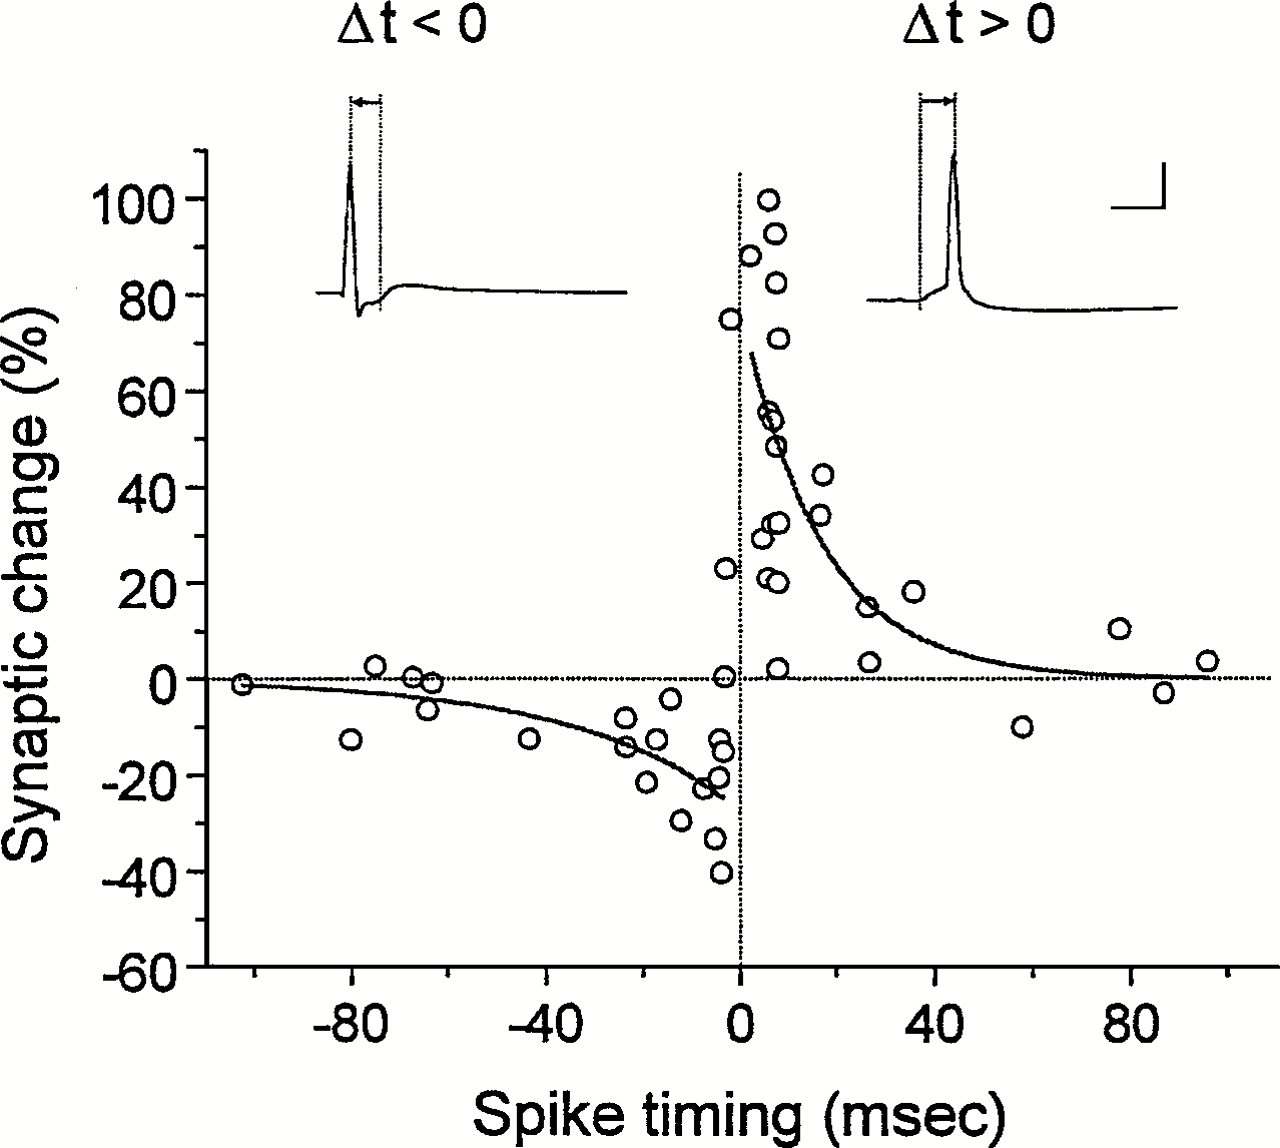
\includegraphics[width=0.5\textwidth]{pics_snn/stdp.jpeg}
	\caption{Synaptic time dependant plasticity~\cite{bi2001synaptic}.
	The circles record the synaptic weight change of real biological observations on 60 pairs of hippocampal neurons.
	Curves of exponential decays against relative timing of pre- and post-synaptic spikes fit well to the real biological data.
	}
	\label{Fig:STDP}
\end{figure}

The synaptic weight is potentiated when a post-synaptic spike fires later than a pre-synaptic spike, and the amplitude of such a potentiation is determined by the curve of exponential decay with a time constant $\tau_+$ and an initial quantity $A_+$;
however, when a post-synaptic spike is generated before a pre-synaptic one, synaptic depression will occur according to the exponential decay defined by $\tau_-$ and $-A_-$.

Besides the standard STDP model~\cite{song2000competitive}, also known as the additive model, stated in Equation~\ref{equ:stdp}, variations of the STDP learning rule have been proposed to satisfy different learning speeds and classification accuracy.
Multiplicative STDP~\cite{morrison2008phenomenological} is an alternative model where the weight change is not only dependant on the relative timing, but also on the current synaptic efficacy:
\begin{equation}
\left\{
\begin{aligned}
A_+ (w) &=  (w_{max} - w)\eta_+~~, \\
A_- (w) &= w\eta_-~~,
\end{aligned}
\right.
\end{equation}
where $A_+$ and $A_-$ in Equation~\ref{equ:stdp} become functions of variable 
$w$, $\eta_+$ and $\eta_-$ define the learning rate of the weight potentiation and depression, and $w_{max}$ is the maximum synaptic efficacy while 0 is the minimum.

We use the multiplicative STDP model for SNN training in Section~\ref{sec:test}, and a much simplified version of asymmetric rectangular STDP in Chapter~\ref{cha:sdlm} where the STDP window is just a constant:
\begin{equation}
\Delta w = \left\{
\begin{aligned}
&\eta \textrm{~,~~when~~~} 0 \leq \Delta  t \leq \tau_{win}\\
& 0 \textrm{~,~~otherwise}.
\end{aligned}
\right.
\end{equation}

\section{Simulating Networks of Spiking Neurons}
\label{sec:snn_sim}
In the last section, we have described neural dynamics is abstracted by mathematical models at the neuronal level.
However, it is challenging to simulate a large SNN with a high volume of synaptic connections, even using simple models like LIF, because of the high event rate ($10^4$ synaptic events per second per single neuron on average).
Addressing this problem, existing solutions vary from software simulators to hardware neuromorphic systems.
%discuss the closed-loop, standing alone neuromorphic systems built on SpiNNaker for real-time cognitive applications.

\subsection{Software Simulators}
Existing approaches to software simulation can be seen as: `clock-driven' where the neural state is updated in some static time resolution, or `event-driven' where the membrane potential is only modified when a spike arrives.
The synchronous `clock-driven' method uses numerical integration for solving ordinary differential equations (ODE), the evolution functions of membrane potential with respect to time.
However, modifications only on the time clocks (usually in 1~ms resolution), the non-linear differential equations can only be approximated rather than solved, and the spike times lose precision since they are bounded to discrete time steps.
`Event-driven' approaches, in comparison, are accurate since they use explicit solutions of the ODEs and the spike arrival time is not rounded to time bins.
Unfortunately, except for LIF neurons, all the other models stated in Section~\ref{subsec:neuron_model} are unsolvable.
In addition, compared to sparse events high synaptic event rate ($10^4$ Hz per neuron) takes no advantage of computational efficiency using this asynchronous approach.
Therefore, most of the popular software simulators use a `hybrid' solution, such as NEST~\cite{gewaltig2007nest} and Brian~\cite{goodman2008brian}, where 
neural state is updated synchronously, but the synapse operates in an event-based way.

Another software tool, PyNN~\cite{davison2008pynn}, is a description language for building SNNs;
it abstracts away the detail of various simulators and provides unified APIs for any simulator that supports it.
Consequently, neuroscientists and SNN designers do not need to learn different `languages' for specific simulators, and the models written in PyNN are supposed to run freely on the supporting simulators.

Most of the SNN models developed in the thesis are described in PyNN and ran on NEST, and some of them are also tested on a hardware simulator, SpiNNaker, which will be introduced in the following section.
In Chapter~\ref{cha:sdlm} we develop our own SNN simulator to implement and test a proposed learning algorithm, and the simulator follows the synchronous convention due to its programming simplicity and flexible neural models selections. 

\subsection{Neuromorphic Hardware}
\label{subsec:neuromorphic_hw}
%TODO can be reworded more logical
Neuromorphic systems can be categorised as analogue, digital, or mixed-mode analogue/digital, depending on how neurons, synapses and spike transmission are implemented. %VLSI circuits. 

Some analogue implementations exploit sub-threshold transistor dynamics to emulate neurons and synapses directly in hardware~\cite{indiveri2011neuromorphic} and are more energy-efficient while requiring less area than their digital counterparts~\cite{joubert2012hardware}.
However, the behaviour of analogue circuits is hard to control through the fabrication process due to transistor mismatch~\cite{indiveri2011neuromorphic,pedram2006thermal,linares2003compact}, and achievable necessary wiring densities render direct point-to-point connections impractical for large-scale systems.

The majority of mixed-mode analogue/digital neuromorphic platforms, such as the High Input Count Analog Neural Network (HI-CANN)~\cite{schemmel2010wafer}, Neurogrid~\cite{benjamin2014neurogrid}, and HiAER-IFAT~\cite{yu201265k}, use analogue circuits to emulate neurons and digital packet-based technology to communicate spikes as Address-Event Representation (AER~\cite{lazzaro1995multi}) events.
This enables reconfigurable connectivity patterns, while spike timing is expressed implicitly since typically a spike reaches its destination in less than a millisecond, thus fulfilling the real-time requirement.

Digital neuromorphic platforms such as TrueNorth~\cite{merolla2014million} use digital circuits with finite precision to simulate neurons in an event-driven manner to minimise the active power dissipation.
Such systems suffer from limited model flexibility, since neurons and synapses are fabricated directly in hardware with only a small subset of parameters under the control of the researcher.
The SpiNNaker many-core neuromorphic architecture~\cite{furber2014spinnaker} uses low-power programmable cores and scalable event-driven communications hardware allowing neural and synaptic models to be implemented in software.
While software modelling provides great flexibility, digital platforms generally have reduced precision (due to the inherent discretisation) and higher energy consumption when compared to analogue platforms.
%Furthermore, the processing cores used in SpiNNaker chips perform better when using integer or fixed-point arithmetic~\cite{Hopkins2015Accuracy}.
%Moreover, the requirement for real-time operations leads to constraints on the complexity of model that can be supported.

\subsection{Neuromorphic Sensory and Processing Systems}
\label{sec:morph}
%\subsubsection{Neuromorphic Sensors}
Neuromorphic engineers have successfully produced visual and auditory silicon devices mimicking the biological retina and cochlea, and boosted the applications of spike-based sensory processing in artificial vision and audition.

The visual input is captured by a DVS (Dynamic Visual Sensor) silicon retina~\cite{serrano2013128, delbruck2008frame}, which is quite different from conventional video cameras.
Each pixel generates spikes when its change in brightness reaches a defined threshold;
thus, instead of buffering video into frames, the activity of pixels is sent out and processed continuously with time.
The communication bandwidth is therefore optimised by sending activity only, which is encoded as pixel events using AER~\cite{lazzaro1995multi} protocol.
The level of activity depends on the contrast change; pixels generate spikes faster and more frequently when they are subject to more active change.
The sensor is capable of capturing very fast moving objects (e.g., up to 10 K rotations per second), which is equivalent to 100 K conventional frames per second~\cite{lenero20113}.

The binaural silicon cochlea~\cite{5537164} models the elementary functions of the cochlea including the basilar membrane, the inner hair cells~(IHCs), and the spiral Ganglion Cells (SGCs).
The input sound wave of each cochlea is filtered by a 64 channel bank of cascaded filters to model the frequency distribution along the basilar membrane.
IHCs locating at each frequency channel perform approximately as half-wave rectifiers, since they release neurotransmitter only when their stereocilia bend   in one direction driven by the membrane potential.
The transformation from mechanical waves to electrical action potentials completes at the spiral SGCs, where four pulse-frequency modulators at each frequency channel act like SGCs and generate spikes with individual thresholds.


The output spikes from the sensory devices are then communicated to back-end SNN processing using the asynchronous AER protocol.
Visual/auditory recognition on such complete neuromorphic hardware systems have emerged in pursuing of efficient energy cost and low sensory latency.
However, these hardware SNN simulators either running on FPGAs~\cite{neil2014minitaur, kiselev2016event} or analogue circuits~\cite{qiao2015reconfigurable} are limited to the current scale.

	\begin{figure}[tbp!]
	\centering
	\begin{subfigure}[t]{0.8\textwidth}
		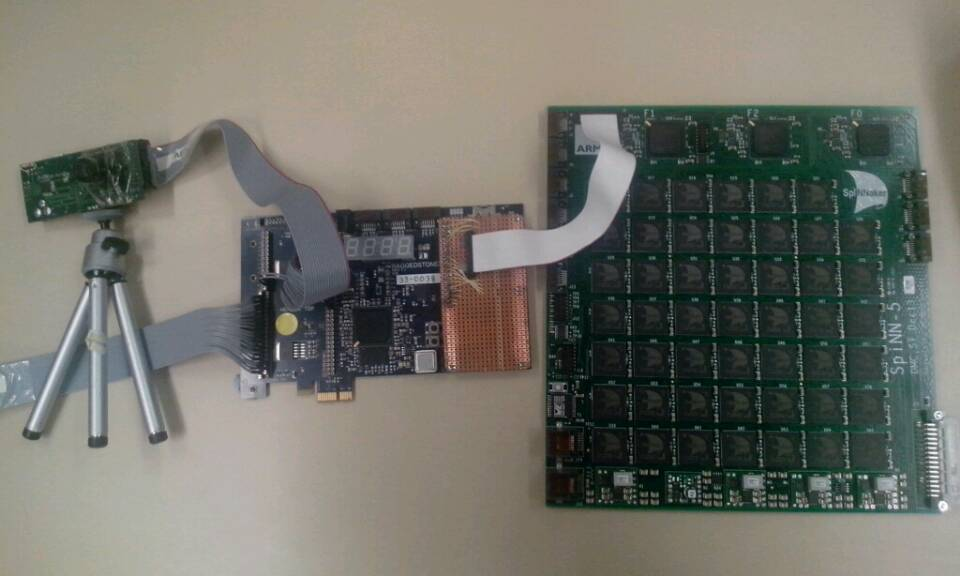
\includegraphics[width=\textwidth]{pics_snn/outline2.jpg}
		\caption{Picture of the neuromorphic visual processing platform. From left to right: a silicon retina, an FPGA board which converts AER packets to SpiNNaker format, and a 48-node SpiNNaker system.}
	\end{subfigure}\\
	\begin{subfigure}[t]{0.528\textwidth}
		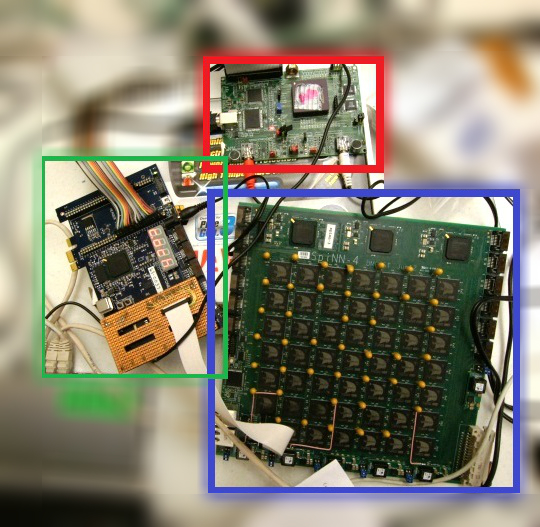
\includegraphics[width=\textwidth]{pics_snn/photooutline_blurred.jpg}
		\caption{Picture of the neuromorphic auditory processing platform which is similar to (a) that a silicon cochlea (up) connects to SpiNNaker board (lower right) through an FPGA (left).}
	\end{subfigure}
	~~
	\begin{subfigure}[t]{0.4\textwidth}
		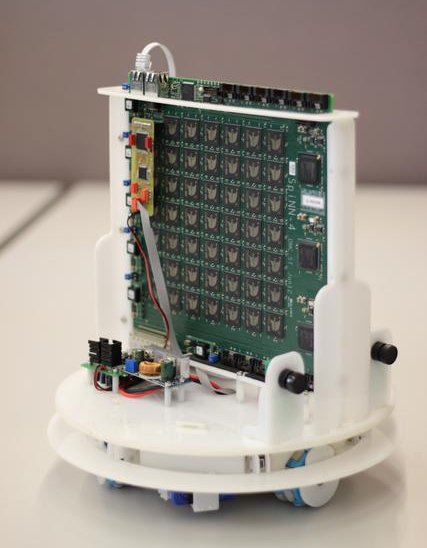
\includegraphics[width=\textwidth]{pics_snn/omnibot.jpg}
		\caption{Picture of the omni-directional platform with embedded low-level motor control and elementary sensors: stereo silicon retinas, wheel encoders, and a bump-sensor ring.}
	\end{subfigure}
	\caption{Three set-ups of neuromorphic sensory and processing hardware platform using SpiNNaker~\cite{furber2014spinnaker}.}
	\label{Fig:close-loop}
\end{figure}

SpiNNaker provides an ideal platform for real-time visual/auditory processing with large SNN models.
Figure~\ref{Fig:close-loop} shows three set-ups of such `standing-alone' neuromorphic sensory and processing hardware platform, which can be operated on its own as a closed-loop system (Figure~\ref{Fig:close-loop}(c)).
The visual system, shown in Figure~\ref{Fig:close-loop}(a), ran a 5-layered SNN model~\cite{liu2014real} we designed for live gesture recognition, which contained a network of 74,210 neurons and 15,216,512 synapses, used 290 SpiNNaker cores in parallel and reached 93.0\% accuracy. 
We also successfully implemented a sound localisation model of spiking neurons on an auditory system, see Figure~\ref{Fig:close-loop}(b), which could operate input spikes with sub-millisecond resolution~\cite{lagorce2015breaking}.
These works prove that real-time, large-scale, sensory neuromorphic systems are ready for further study on effective cognition and genuine intelligence of such biological-plausible machines.

\section{Summary}
This chapter introduced the structure and behaviour of biological neurons and illustrated how these neural dynamics can be modelled by mathematical abstractions as spiking neurons, which are the basic components of an SNN.
The difference between biologically-plausible spiking neuronal operations and rate-based artificial activations holds the key to the research question: How to equip SNNs with cognitive capabilities equivalent to ANNs.
Finally, we give an overview of all the tools and hardware platforms, which are used later in the thesis, for SNN simulations.
